\documentclass{article}
\usepackage{lingmacros}
\usepackage[margin=1.7in]{geometry}
\usepackage{graphicx}
\usepackage{hyperref}
\hypersetup{colorlinks=true,linkcolor=blue, linktocpage}
\graphicspath{ {./img/} }
\begin{document}
\author{Benjamin Barda, Francesco Danese, Alessandro Vecchi}
\title{\vspace{-2cm}\textbf{Self-Supervised meets Active-Learning}}
\maketitle

\section{Introduction}
\begin{flushleft}
While Data is getting generated at an ever increasing speed and can be retrieved with not much effort,
making this data useful and usable is still not a trivial task at all.
One of the main bottlenecks is the need of vast amount of labeled data, which, for a high quality dataset,
needs to be manually labeled with care, a process that requires a lot of man-hours to complete. 
This is the foundamental problem that researchers in the field of Active Learning are trying to answer. 
How can we get competitive performance with less data?
\end{flushleft}
\begin{flushleft}
The core idea of Active Learning is to get more out of the human in the loop.
But how can we do this?
Clearly is not possible to force someone to annotate faster, but what we can do is make sure 
that every sample that he labels have as much impact as possible, by selecting those with higher \emph{uncertainty} .


\begin{figure}[h]
    \centering
    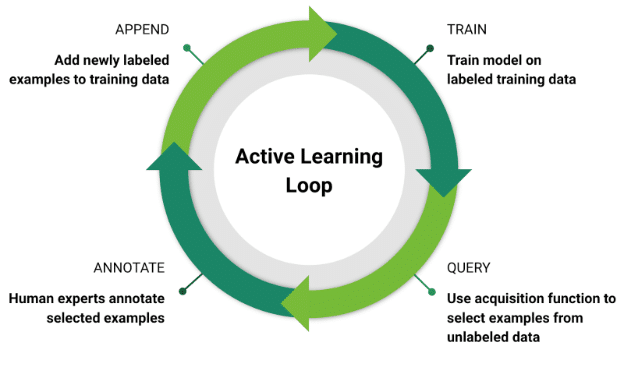
\includegraphics[scale=0.5]{AL-loop}
\end{figure}

The process is relatively simple from an overview perspective.

Starting from an existing dataset of unlabeled data we select via an acquisition 
function the \emph{most informative} samples to be presented to the oracle (a human expert for example) 
for he to annotate them and add them to the labeled dataset. We then train the model on the labeled data. 
We repeat this process until exhausting the labelling budget (time, money, ecc..).
\section{Measuring uncertainty}
\label{sec:entropy}
\subsection{Acquisition functions}
To know how much the model is certain about the prediction it makes for a given sample, 
we need some kind of function the takes into consideration the output of the model for that particular sample.
Lets look at a few classic uncertainty acquisition functions:
\begin{enumerate}
    \item Entropy: $H(p) = - \sum{p_iLog_2(p_i)}$ where $p_i$ is the probability the model outputs for class \emph{i}, 
    refering for instance to the last softmax layer of a NeuralNet.
    H will grow as the probabilities p tend to be more uniform, and will shrink when fewer of the categories tend to get higher values.
    \item Variation ratio: $1 - max(p)$
    \item The difference between the largest output from the model, and the second largest output.
    \item In SVMs: the distance of a point from the hyperplane.
\end{enumerate}
\subsection{Query by Committee QBC}
Another concept from classical active learning papers, is QBC. 
The idea here is that instead of measuring the uncertainty of a single model, 
we can train an ensemble of many different models (maybe with different seeds, 
or hyper-parameters, or structures). Then for a given image, 
we can check if the output changes a lot between models. If it does, 
it means the models aren’t very consistent about this image, 
and some of them aren’t doing a good job on this image.
\section{Active Learning: Not only one way}
There are three main approaches to the problem :
\begin{itemize}
    \item Stream based selective sampling
    \item Pool-Based sampling
    \item Membership query synthesis
\end{itemize}
In this project we investigare Pool-Based sampling but for an overview of the various methods \href{https://www.datarobot.com/blog/active-learning-machine-learning/}{this article} might be a good starting point.
\begin{flushleft}
    Our approach can be divided in two main steps:
\end{flushleft}
\begin{itemize}
    \item Pretrain
    \item Active learning loop
\end{itemize}

\subsection{Pretrain}
This is a crucial part of the method proposed, in fact the quality of the features learned 
during this phase have a great impact on the final performnace, 
so we put great consideration in selecting the appropiate pretext task.

The one thing that remained constant during all of our experiments 
were was the choice of the architechture. 
We decided to use a Residual Network for two reasons:
\begin{enumerate}
    \item Low number of learnable parameters
    \item Proved history of great performance on CIFAR10, the dataset we chose for this project.
\end{enumerate}
\begin{figure}[h]
    \centering
    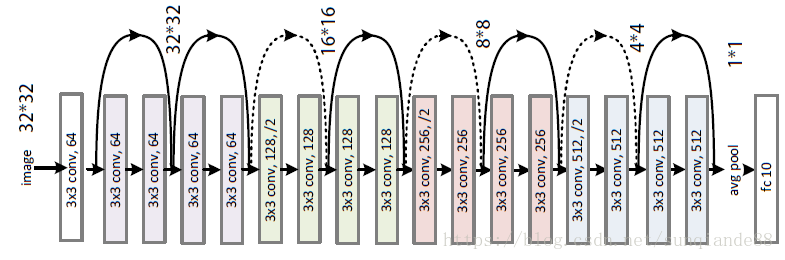
\includegraphics[scale=0.46]{resnet18}
    \caption{ 18 layers Residual Network architecture. }
\end{figure}
During the first phase of the project we considered using the non constrastive task 
described in SimSiam. Even though the quality of the features were excellent 
we faced the problem of limited resources in terms of computing and time, 
and since to have an effective pretrain we would need to run at least 800 epochs 
we decided to discard this option.
\end{flushleft}
\begin{flushleft}
We then resorted to a simpler task, more specifically \emph{rotation prediction}, 
as described in the RotNet paper.
\end{flushleft}
\subsection{Self supervised task: Predicting rotations}
\begin{flushleft}
Supervised feature learning has the main limitation of requiring intensive manual labeling effort, which is both expensive and
infeasible to scale on the vast amount of visual data that are available today.
Due to that, there is lately an increased interest to learn high level ConvNet based representations
in an unsupervised manner that avoids manual annotation of visual data.
Among them, a prominent paradigm is the so-called self-supervised learning that defines an annotation free pretext task,
using only the visual information present on the images or videos, in order to provide a surrogate
supervision signal for feature learning.
\end{flushleft}
\begin{flushleft}
    \begin{figure}[h]
        \centering
        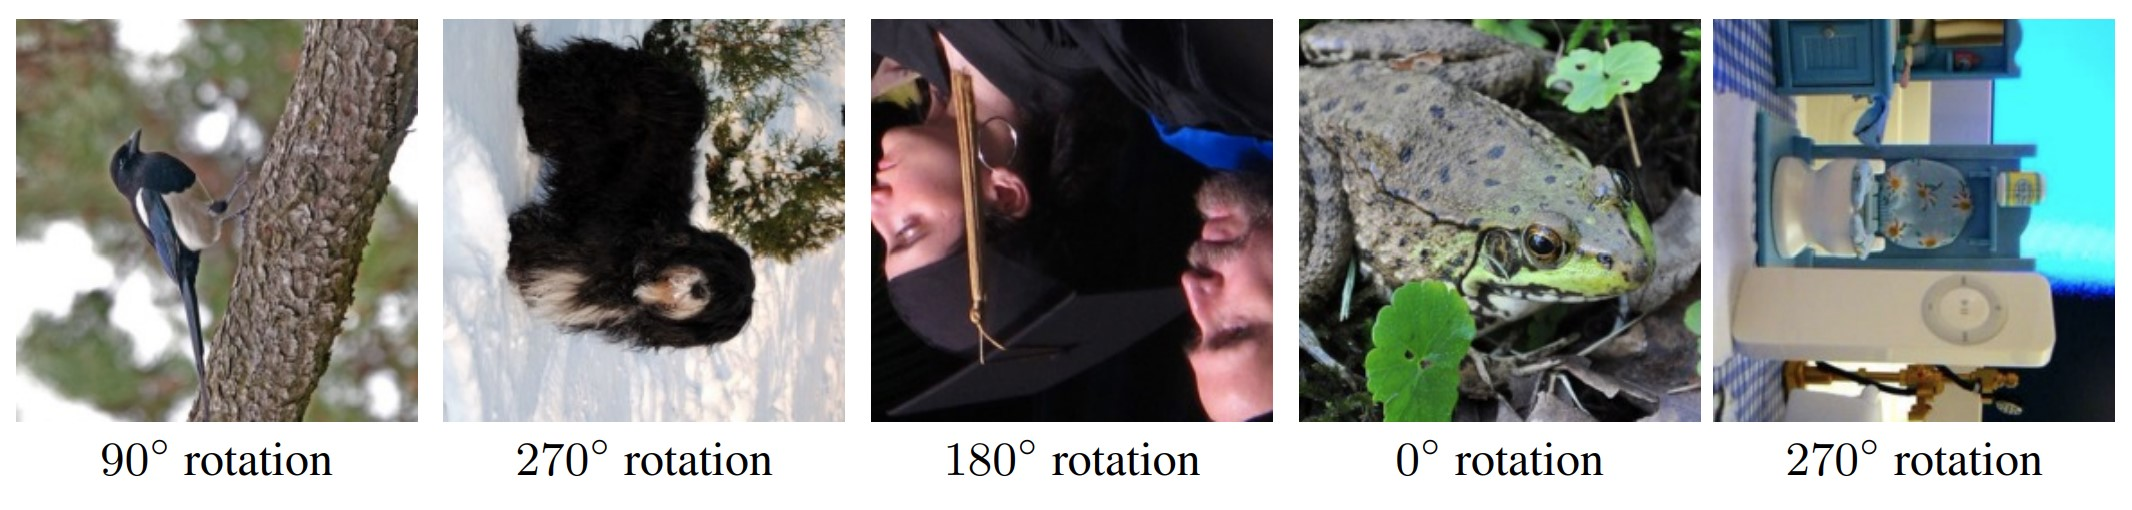
\includegraphics[scale=0.45]{rotations}
        \caption{ Transformations applied to some input images. }
    \end{figure}
Our work follows the self-supervised paradigm and learn image representations by training the network to recognize the geometric transformation that is applied to the image that it gets as
input.
Those transformations are the image rotations by 0, 90, 180, and 270 degrees. Thus,
the ConvNet model is trained on the 4-way image classification task of recognizing one of the four
image rotations. The idea is that in order to be able to recognize the
rotation transformation that was applied to an image the model will be required to understand the concept of
the objects depicted in the image, such as their location in the image, their type, and
their pose.
\end{flushleft}
\begin{flushleft}
The big advantage over the SimSiam approach is the realative low number of epochs it needs. 
In fact around 100 epochs are needed to have an effective pretrain, allowing us to complete the training in a 
single colab session in less than 2 hours.
\subsection{Pretrain Results}
\begin{figure}[h]
    \centering
    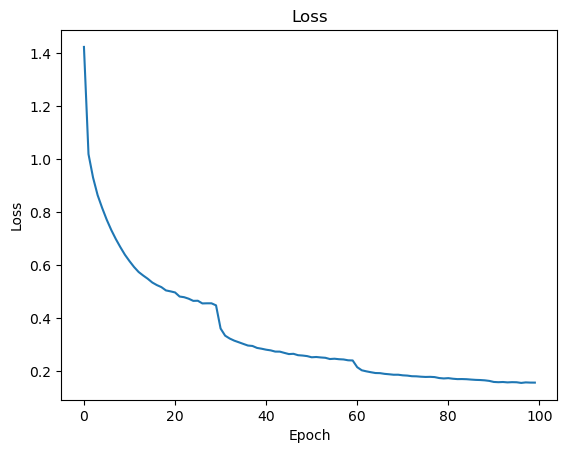
\includegraphics[scale=0.63]{pretrain_loss}
    \caption{ Pretrain loss during learning phase. }
\end{figure}
The loss function that we used, since we are dealing with classification, is the classic Cross Entropy Loss: $ -\sum_x{p(x)Log(q(x))}$ where $x \in classes$, $p(x)$ is the true probability (one hot encoded) and 
$q(x)$ is the predicted probability. After 100 epochs with data batches of size 512 the loss was around 0.2, optimized via Adam Gradient Descent and Cosine Annealing scheduler for the adaptive learning rate with 0.3 as starting value.
The final accuracy on the evaluation set reached 0.89 on the 4-class prediction task.
\begin{figure}[h]
    \centering
    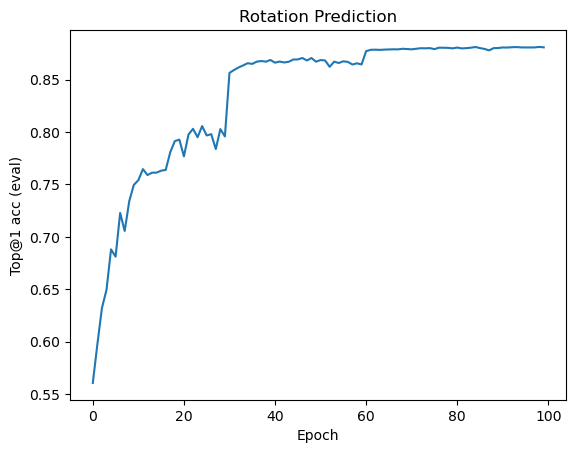
\includegraphics[scale=0.65]{pretrain_acc}
    \caption{ Pretrain accuracy during learning phase.}
\end{figure}
\subsection{Active learning loop}
Once the pretrain stage is finished it's time to focus on the actual classification task.
 For doing so we have discarded the final 4-outputs layer and attached a simple Linear Classifier in place of it, 
that maps 512 nodes to 10 softmaxed nodes representing the classes.
So the model to train now is the previous ResNet18 with a Logistic Regression mounted at the end of it, and the whole structure is 
ready to be fine-tuned on the new task with the help of the active learning method.
We started with 20\% of the training set and linearly added the sample selected by the model every 50 epochs, until 50\% of the training set size was reached. The model requested the new labelled samples
using \hyperref[sec:entropy]{Entropy} as Acquisition function. Notice, on the plots, the sudden "jumps" of loss and accuracy values at the instants new samples were added.
\begin{figure}[h]
    \centering
    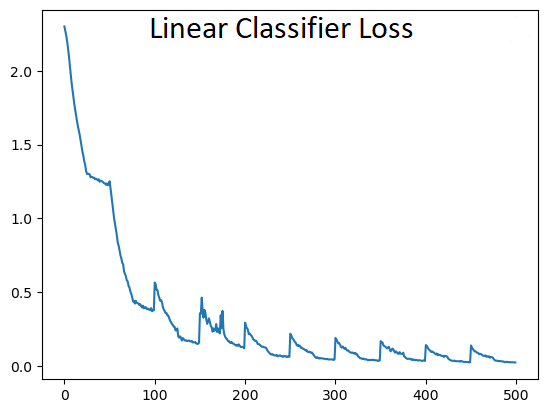
\includegraphics[scale=1.25]{lcsl_500_20_50_loss}
    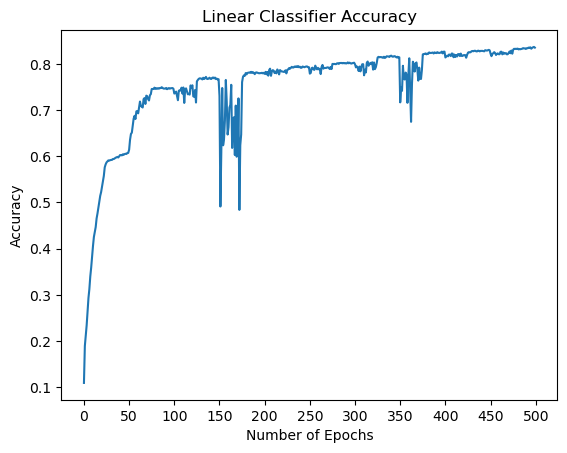
\includegraphics[scale=0.65]{lcsl_500_20_50_acc}
    \caption{Loss (above) and accuracy (below) of pretrained ResNet + linear classifier on CIFAR10 over active learning training epochs}
\end{figure}
\end{flushleft}
\end{document}